\documentclass[10pt,twocolumn]{article}
\usepackage[utf8]{inputenc}
\usepackage[ spanish]{babel}
\usepackage{graphicx}
\usepackage{url}
\usepackage[hidelinks]{hyperref}
%\usepackage[round]{natbib} %Para soportar las referencias con nombre de autor y año


%\usepackage[pdflang=es-MX]{hyperref}

\title{Stomatopoda}
\author{Eduardo René Rodríguez Ávila}

\begin{document}
\maketitle

Los \textbf{estomatópodos} (Stomatopoda) son un or\-den de \textbf{crustáceos malacostráceos} del superorden \textit{Hoplocarida}\cite{martin_updated_2001} conocidos comúnmente como galeras, langostas mantis, \underline{mantis marinas}, langostas boxeadoras, esquilas y tamarutacas.

\begin{figure}[h] 
	\centering
	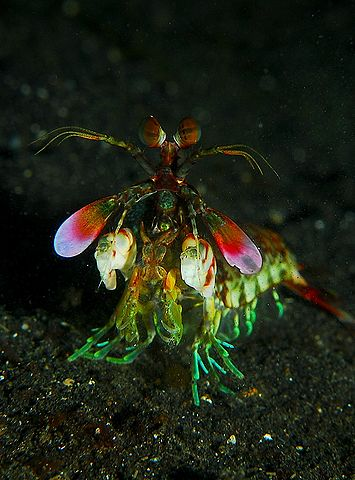
\includegraphics[width=0.2\textwidth]{img/stomatopoda.jpg}
	\caption{\textit{Odontodactylus latirostris} (cabeza)}
\end{figure}

Se les llama mantis por presentar cierto parecido con tales insectos (ver figura 1), en particular unas extremidades anteriores raptoras y el mimetismo\footnote{El mimetismo es una habilidad que ciertos seres vivos poseen para asemejarse a otros organismos (con los que no guarda relación) y a su propio entorno para obtener alguna ventaja funcional}; la capacidad de distinguir la luz polarizada y reaccionar ante ella; el aspecto externo destacado de los ojos y su carácter de depredadores que consumen vorazmente a otros animales. Reciben el nombre de ``boxeadoras'' por que son capaces de ataques rápidos y violentos y se sabe que algunos especímenes han roto de un golpe el cristal del acuario.\cite{holladay_shrimp_2006} Erugosquilla grahami (Ahyong \& Manning, 1998), nativa de los mares de Australia tiene documentada la Marca de 5 mi\-li\-se\-gun\-dos.



Su longitud puede alcanzar hasta 30 o incluso 38 cm\cite{gonser_large_2007}. El caparazón de las mantis marinas cubre la cabeza y los ocho primeros segmentos del tórax por la parte del tergo. Presentan una gran variedad de colores, desde llamativos rojos, naranjas, morados, verdes, blancos, azules hasta marrones y ocres, contando también con pálidos y fluorescentes. A pesar de que son animales comunes y están entre los depredadores más importantes en aguas someras en muchos hábitats marinos tropicales y subtropicales, son poco co\-no\-ci\-dos, ya que muchas especies pasan la mayor parte de su vida escondidas en madrigueras y agujeros.\cite{piper_extraordinary_2007}


\section{Ecología}

Son agresivas y generalmente solitarias y pasan la mayor parte del tiempo escondidas en formaciones rocosas o en madrigueras con pasadizos intrincados, en el fondo del mar. Prefieren esperar a que la presa se acerque de manera azarosa para atacarla y matarla, a diferencia de la mayoría de los crustáceos, que persiguen a la presa. Rara vez salen de sus escondites y pueden ser diurnos, nocturnos o crepusculares, dependiendo de la especie. La mayoría de las especies viven en mares tropicales y subtropicales, como el mar Caribe o los océanos Índico y Pacífico, entre el este de África, Hawai y América tropical, aunque algunas viven en mares templados, como \textit{Squilla mantis}\footnote {La galera (Squilla mantis) es una especie de crustáceo estomatópodo de la familia Squillidae}.

\section{Clasificación y garras
}
Se han descrito cerca de 400 especies de mantis ma\-ri\-nas y todas las especies vivas pertenecen al sub\-or\-den \textit{Unipeltata}\footnote{Stomatopoda. Tree of Life Web Project (1 de enero de 2002) \url{http://tolweb.org/Stomatopoda/6299}}.

Según el tipo de garra, que es usada como arma de ataque y caza se distinguen dos grupos:

\begin{itemize}
	\item  Perforadoras: están armadas con apéndices espinosos rematados con puntas de púas, utilizados para apuñalar y enganchar a las presas (ver figura 2).
	\item Trituradoras: tienen un brazo desarrollado como garrote y una púa rudimentaria (que sin embargo es fuerte y se utiliza en las luchas entre ejemplares de la propia clase). El brazo se utiliza para apalear y aplastar a las presas. La parte interna del dáctilo (la porción terminal) puede poseer un borde afilado, con el que puede cortar la presa mientras nada.
\begin{figure}[h] 
	\centering
	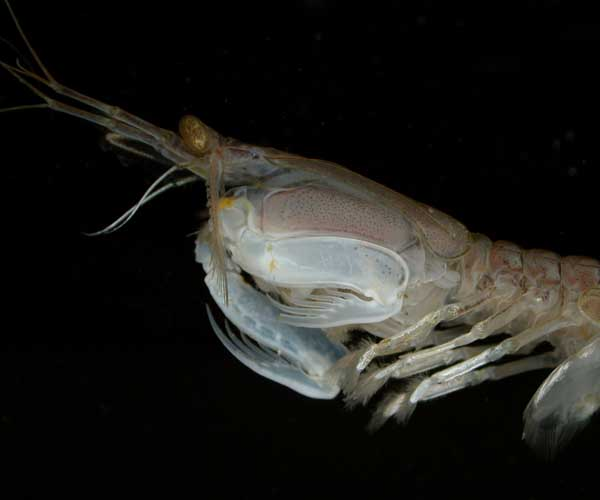
\includegraphics[width=0.2\textwidth]{img/squilla_mantis.jpg}
	\caption{\textit{Squilla mantis}  mostrando sus arpones}
\end{figure}
\end{itemize}

Ambos tipos golpean rápidamente y agitando sus garras rapaces en la presa son capaces de infligir daños graves en víctimas significativamente mayores en tamaño que ellos. Las trituradoras emplean estas armas con rapidez cegadora, con una aceleración de 10,400 G (102,000 m/s$^{2}$, o 335,000 pies/s$^{2}$) y una velocidad de 23 m/s$^{2}$ sin tener que trasladarse\cite{patek_deadly_2004}, equivalente a la aceleración alcanzada por un proyectil calibre 22. Debido a la rapidez del golpe se generan burbujas de cavitación entre el brazo y la superficie golpeada. El colapso de estas burbujas de cavitación produce fuerzas sobre su presa adicionales a las del golpe mismo, de 1,500 newton, lo cual significa que la presa es doblemente golpeada. Aunque el golpe inicial falle, la onda de choque resultante puede ser suficiente para aturdir o hasta matar a las presas.

El golpe también causa sonoluminiscencia a partir del colapso de la burbuja. Esto produce durante un intervalo tremendamente corto una cantidad muy pequeña de luz y una temperatura de miles de grados dentro de la burbuja que colapsa. En estas condiciones los átomos se ionizan y los electrones pasan a formar un plasma que emite luz. Sin embargo las temperaturas se alcanzan en puntos muy localizados y se disipan casi al instante. Tanto la luz como la subida de la temperatura son demasiado débiles y de corta duración para ser detectados sin necesidad de equipos científicos avanzados. La emisión de luz y aumento de la temperatura probablemente no tienen importancia biológica, sino que son meros efectos secundarios del golpe, producto de la cavitación (los crustáceos de la familia Alpheidae producen un efecto similar).

\section{Los ojos}

La región de la banda media del ojo de las mantis marinas (figura 3) se compone de seis hileras de ommatidios especializados. Cuatro de ellas tienen 16 diferentes tipos de pigmentos fotorreceptores, tienen la sensibilidad para diferenciar los colores, los otros filtran el color. Ambos ojos pueden percibir la luz polarizada y poseen visión de color hiperespectral. Cada ojo está sobre una antena móvil independiente del otro, permitiendo a ambos una percepción diferenciada y paralela. Estos ojos presentan variados colores y se considera que permiten una de las visiones más complejas del reino animal.

Cada ojo compuesto está conformado por 10,000 ommatidios y cada uno consta de dos hemisferios aplanados, separados por seis hileras paralelas de omatidios altamente especializados, colectivamente llamados la banda media, que divide el ojo en tres regiones. Las mantis marítimas pueden ver el mismo objeto hasta con tres formas diferentes. En otras palabras, cada ojo posee visión trinocular y percepción de la profundidad. Los hemisferios superior e inferior son usados primariamente para reconocimiento de formas y movimientos y no para visión de color.

Las hileras 1 a 4 de la banda media se especializan en la visión en color, desde el ultravioleta hasta el infrarrojo. Los elementos ópticos de esas filas tienen ocho diferentes clases pigmentos visuales y el rhabdom está dividido en tres diferentes epitelios pigmentarios, cada cual adaptado para diferentes longitudes de onda.

\begin{figure}[h] 
	\centering
	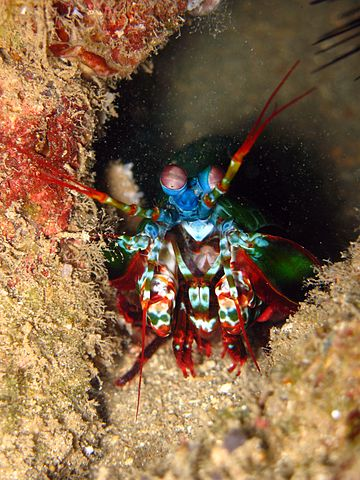
\includegraphics[width=0.2\textwidth]{img/indonesian_mantis_shrimp.jpg}
	\caption{Ojos de una mantis marina en mares de Indonesia}
\end{figure}


\bibliographystyle{unsrt}
\bibliography{referencias2}

Más información en:  \url{http://es.wikipedia.org/wiki/Stomatopoda}
\end{document}
